\section*{CONCLUSÃO}
Neste projeto, percorremos por meio do contexto técnico e social do desenvolvimento dos criptoativos, averiguamos a motivação de desintermediação das atividades financeiras por meio da origem do \textit{Bitcoin}; exploramos o ecossistema cripto por meio dos contratos inteligentes e da \textit{DeFi}, e exibimos seu impacto diante da economia tradicional.

Sob maior incisão teórica no projeto, apresentamos os conceitos chave do funcionamento do \textit{Bitcoin}, constatamos a estrutura dos blocos, a estrutura do encadeamento, o procedimento de prova de trabalho utilizado na mineração do \textit{Bitcoin} e como constitui o seu caráter criptográfico.

Vimos também como a natureza do \textit{Bitcoin}, de maneira programática, corrobora aos conceitos técnico-economicos da Escola Austríaca de Economia, provendo respaldo diante das características do dinheiro, tão bem como as funções da moeda. Apresentamos o resultado da comparação de suas características ao papel-moeda e ao ouros por Fernando Ulrich.

Por fim, atuamos na experimentação educacional da implementação de um sistema de \textit{blockchain} de nível médio, que abstrai os conceitos base do \textit{Bitcoin}, permite a manipulação via requisições e exibe as classes presentes da corrente no navegador. Foi exposto todas as estruturas geradas neste experimento, seus atributos e suas funções diantes da rede.

\section*{Exibição do Experimento de \textit{Blockchain} em Rust}
Nas Figuras a seguir constam as imagens desta experimentação, o repositório onde o código e os arquivos deste teste foram armazenados na plataforma Github por preferência dos autores. O código se encontra disponível por este link:
\href{https://github.com/HeberUnifil/Educational-Blockchain-Currency}{\textcolor{blue}{https://github.com/HeberUnifil/Educational-Blockchain-Currency}} .

Na Figura \ref*{fig:terminal} consta o registro via terminal Linux das atualizações realizadas na \textit{Blockchain}:

\begin{figure} [h]
	\centering
	\caption{Resposta via terminal sobre as atualizações na \textit{Blockchain}.}
	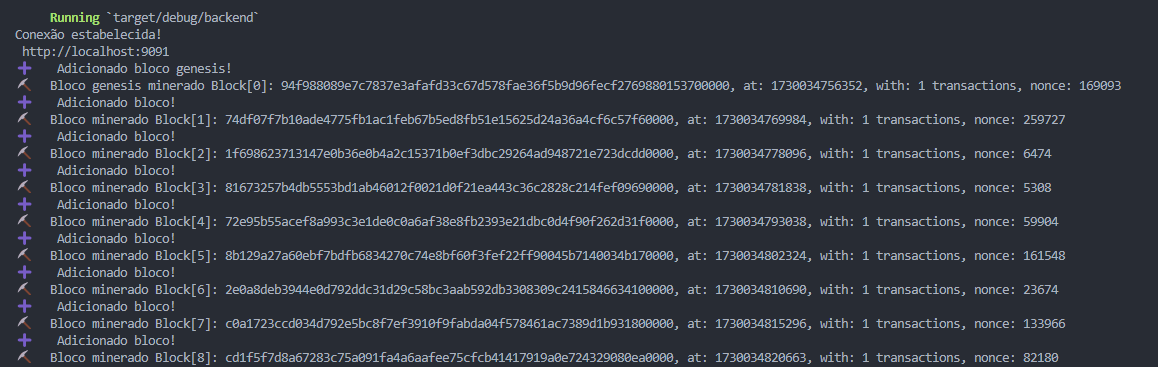
\includegraphics[width=1\linewidth]{../images/terminal-blockchain.png}
	\label{fig:terminal}
	\text{Fonte: Captura de tela tirada pelos autores}

\end{figure}

Na Figura \ref*{fig:navegador} consta a exibição geral dos blocos ordenados na corrente, seus respectivos \textit{hashes}, sua marca temporal, quantidade de transações e o número de tentativas para mineração do bloco.

\begin{figure} [h]
	\centering
	\caption{Resposta via terminal sobre as atualizações na \textit{Blockchain}.}
	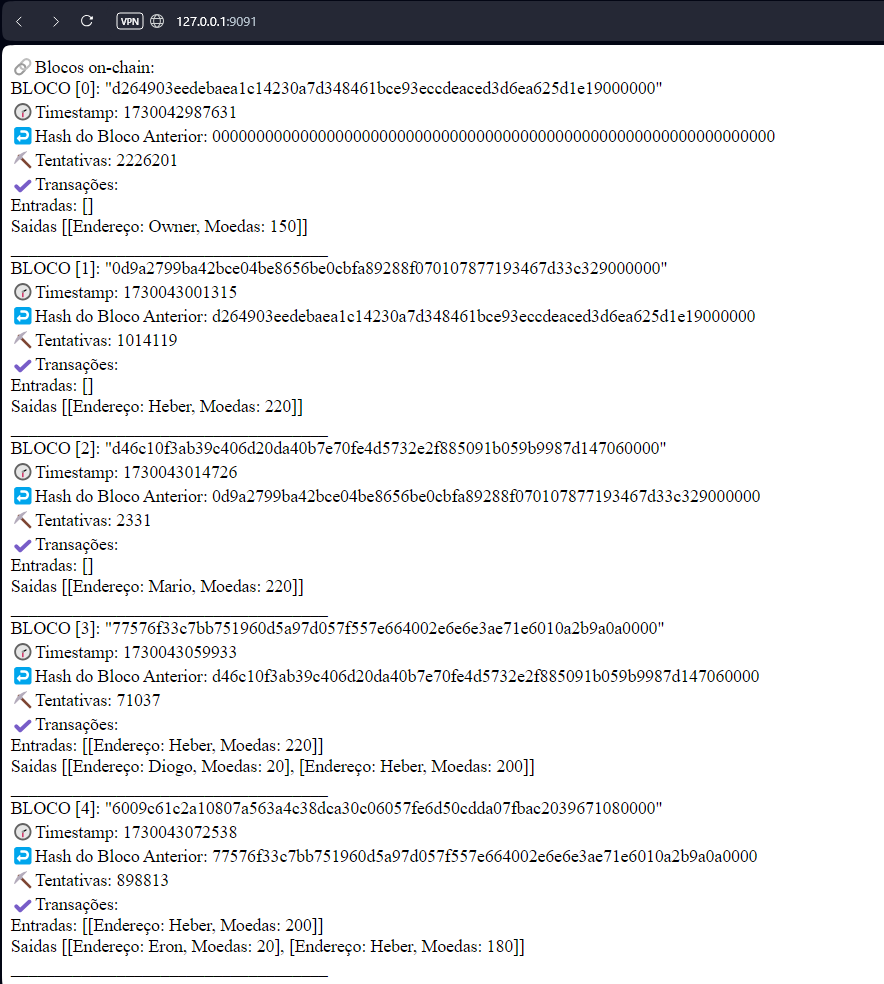
\includegraphics[width=1\linewidth]{../images/navegador-blockchain.png}
	\label{fig:navegador}
	\text{Fonte: Captura de tela tirada pelos autores}

\end{figure}

% \begin{figure} [h]
% 	\centering
% 	\caption{Resposta via terminal sobre as atualizações na \textit{Blockchain}.}
% 	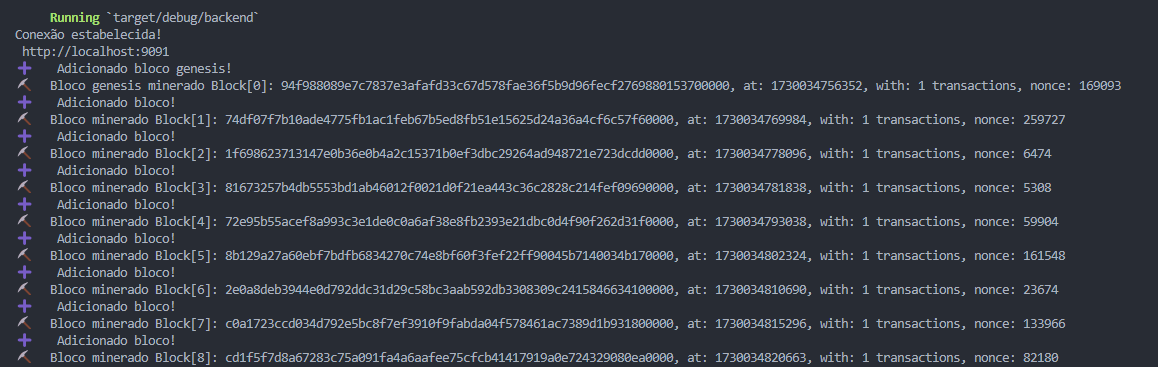
\includegraphics[width=.8\linewidth]{../images/terminal-blockchain.png}
% 	\label{fig:terminal}
% 	\text{Fonte: Captura de tela tirada pelos autores}

% \end{figure}